\begin{formal}
På figurer er det veldig viktig å ta med N, dvs. hvor mange datapunkter er det i materialet totalt.
På histogram der man forventer at leseren skal vurdere histogram mot hverandre er det viktig at aksene har samme utstrekning og at alle datapunkter for alle grupper er innenfor aksene. I histogram er det gjerne frekvenser (dvs. antall på Y aksen) men det er fult mulig å produsere histogram som har andel på Y aksen og da blir det enklere å sammenlikne histogram.
\end{formal}

Figurene nedenfor viser de (vaskede) totalvektene fra prøveordningen fremstilt som histogrammer.
X-aksen er trimmet til det samme intervallet for samtlige ekvipasjer, og samtlige illustrasjoner er
supplert med $N$: antallet datapunkter illustrasjonen består av.

\begin{figure}[H]
    \centering
    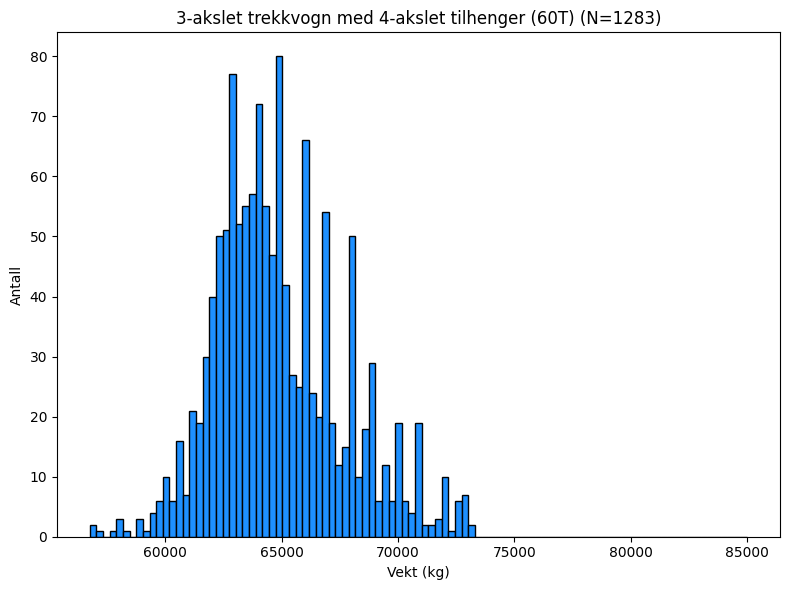
\includegraphics[width=0.75\textwidth]{images/n60.png}
    \caption{Analyse av transportarbeid for ulike ekvipasjer}
    \label{fig:n60}
\end{figure}

\begin{figure}[H]
    \centering
    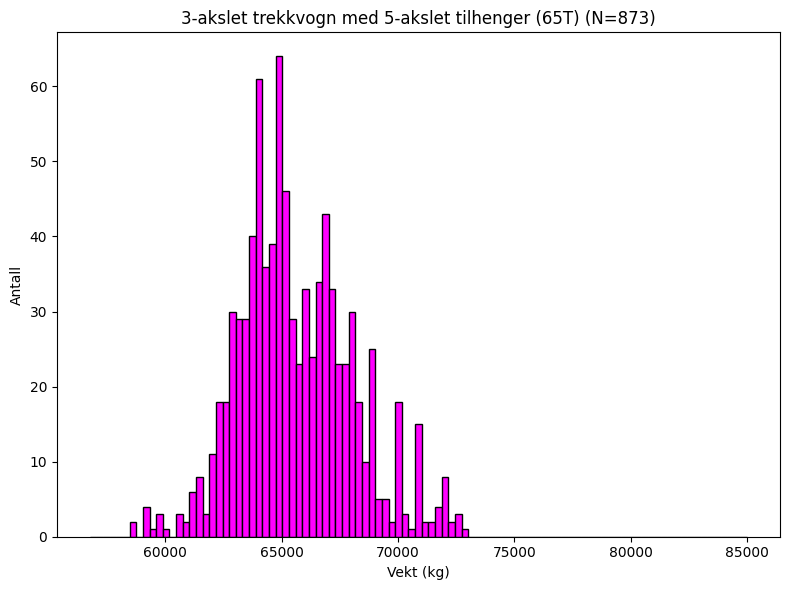
\includegraphics[width=0.75\textwidth]{images/n65.png}
    \caption{Analyse av transportarbeid for ulike ekvipasjer}
    \label{fig:n65}
\end{figure}

\begin{figure}[H]
    \centering
    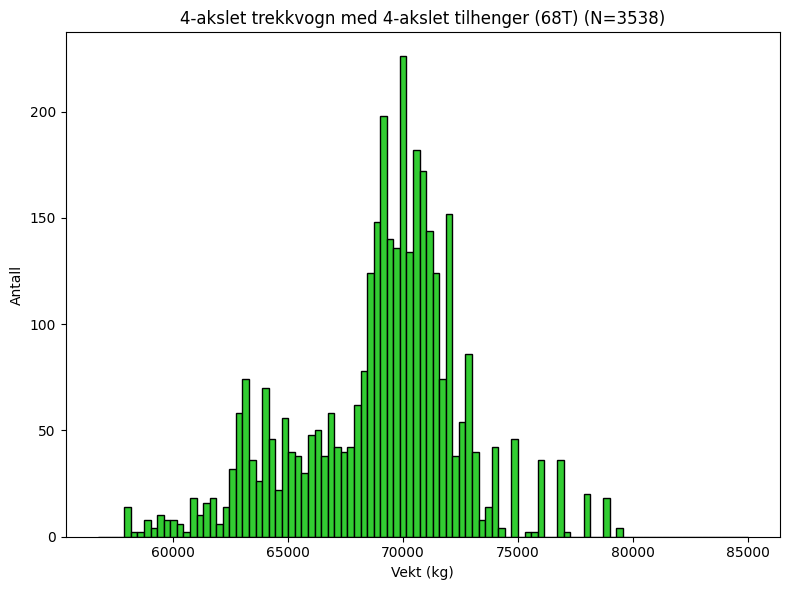
\includegraphics[width=0.75\textwidth]{images/n68.png}
    \caption{Analyse av transportarbeid for ulike ekvipasjer}
    \label{fig:n68}
\end{figure}

\begin{figure}[H]
    \centering
    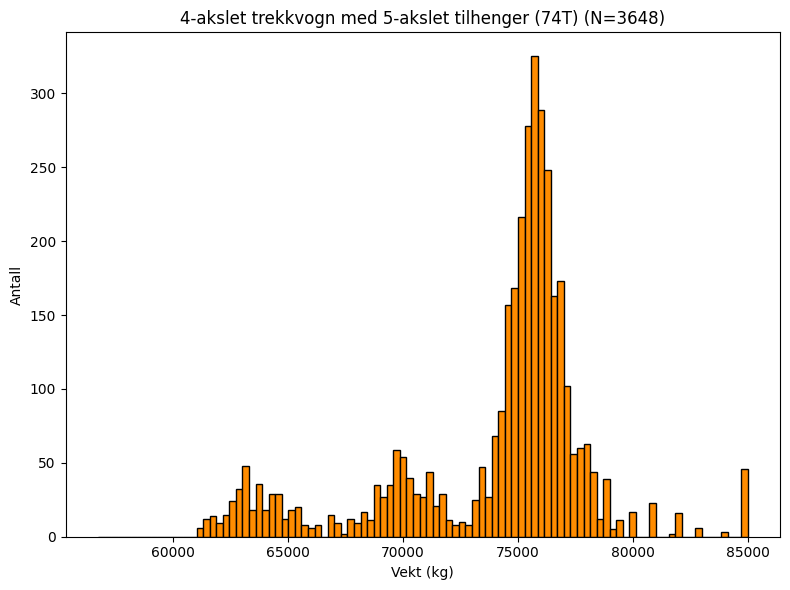
\includegraphics[width=0.75\textwidth]{images/n74.png}
    \caption{Analyse av transportarbeid for ulike ekvipasjer}
    \label{fig:n74}
\end{figure}
